\documentclass[aspectratio=169]{beamer}
\usetheme{Madrid}
\usepackage[utf8]{inputenc}
\usepackage[T1]{fontenc}
\usepackage{tikz}
\usepackage{amssymb}
\usepackage{graphicx}
\setbeamertemplate{navigation symbols}{}
\setbeamercolor{title}{fg=white,bg=green!55!teal}
\setbeamercolor{frametitle}{fg=white,bg=green!55!teal}
\setbeamercolor{block title}{bg=green!55!teal!20,fg=black}
\setbeamercolor{block body}{bg=green!55!teal!8,fg=black}
\setbeamercolor{item}{fg=green!55!teal}
\setbeamercolor{itemize item}{fg=green!55!teal}
\setbeamertemplate{itemize item}[triangle]

\title{M7 — Inside the Machine}
\subtitle{Binary numbers, storage units, how images/sound are numbers}
\author{ByteForge --- Grade 8 --- App Builder}
\date{}

\begin{document}

\begin{frame}
    \titlepage
\end{frame}

\begin{frame}{Today's Plan}
    \begin{itemize}
        \item Storage Units \& Binary
        \item Images Are Numbers
        \item Interpreter vs. Compiler
        \item Encoding \& Decoding
        \item Run-Length Encoding
        \item[$\bigstar$] BOSS --- M7 Capstone
    \end{itemize}
\end{frame}

\begin{frame}{1024, not 1000 — powers of two}
    \large
    \begin{itemize}
        \item 1 KB = 1024 bytes, not 1000
        \item Because computers count in binary (base 2), and 1024 is a power of 2. \texttt{bin(42)} reveals the actual binary digits underneath.
    \end{itemize}
\end{frame}


\begin{frame}{Images ARE numbers — grayscale conversion}
    \large
    \begin{itemize}
        \item A colour pixel is a tuple \texttt{(r, g, b)}
        \item \texttt{(r + g + b) // 3} averages the three channels into one brightness number, exactly how a real photo-editing app converts colour to grayscale.
    \end{itemize}
\end{frame}


\begin{frame}{Interpreter vs. compiler}
    \large
    \begin{itemize}
        \item Python is an interpreter
        \item It runs each line as it goes, so everything BEFORE a crash has already genuinely happened. A compiler translates the WHOLE program first.
    \end{itemize}
\end{frame}


\begin{frame}{Run-length encoding — real compression}
    \large
    \begin{itemize}
        \item "aaaabbbccd" stored as "4a3b2c1d" is genuinely shorter
        \item A real compression technique, used in actual image and file formats.
    \end{itemize}
\end{frame}

\begin{frame}{Real-World Examples}
    \large
    \begin{itemize}
        \item Every JPEG/PNG file on your phone is really just numbers, exactly like M7's grayscale pixel maths, just with far more channels and compression on top. Minecraft's own world files are binary data on disk
        \item The same "everything is really numbers" idea, at world-save scale.
    \end{itemize}
\end{frame}


\begin{frame}{Image}
    \begin{center}
    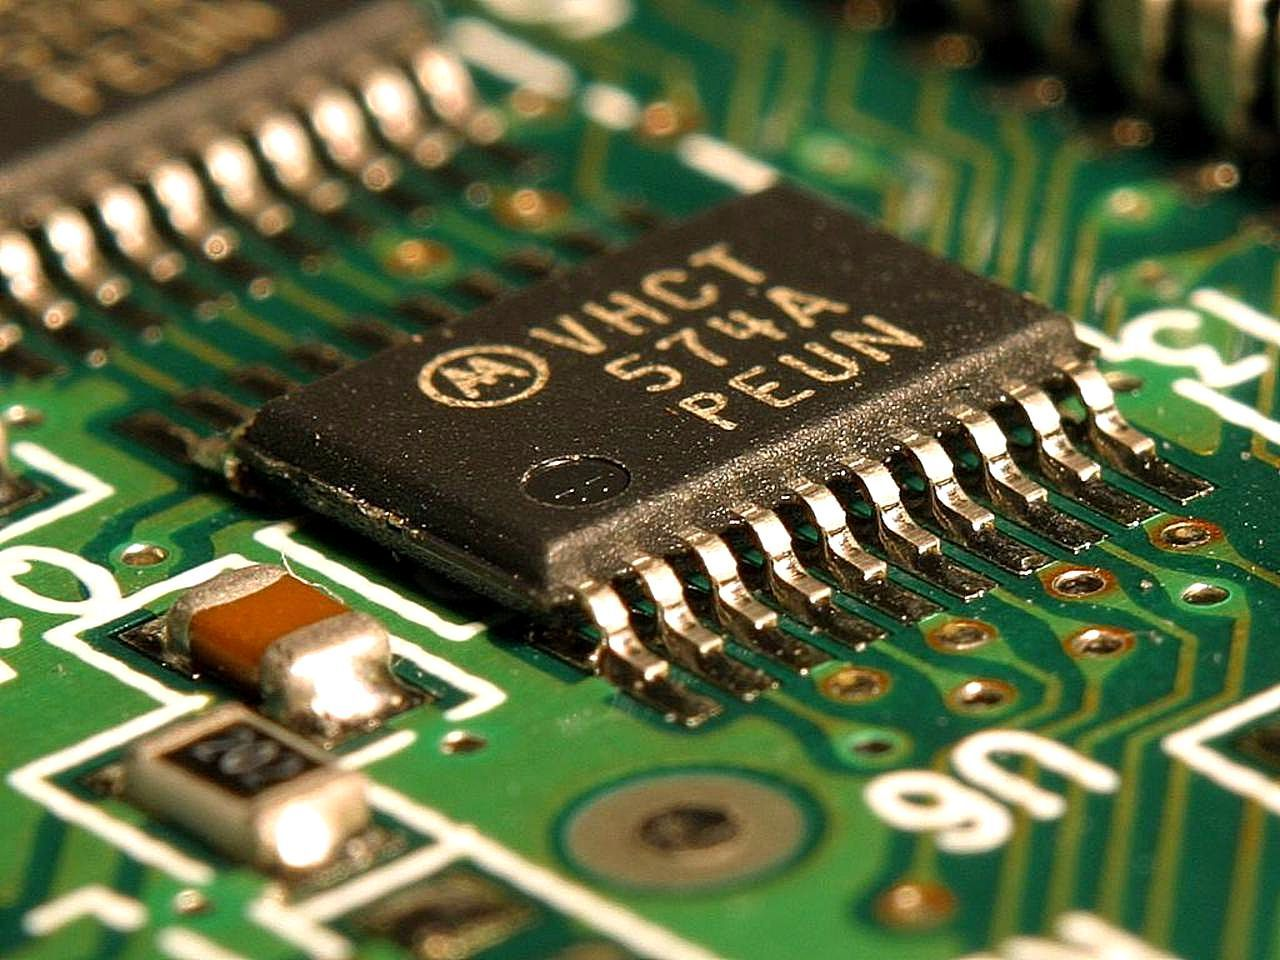
\includegraphics[width=0.5\textwidth]{images/circuit.jpg}

    \large Real transistors and circuits --- what 'inside the machine' actually looks like.

    \small Computer circuit board, Jon Sullivan, public domain, via Wikimedia Commons
    \end{center}
\end{frame}

\begin{frame}{Let Them Discover}
    \Large
    Take any small greyish photo (or imagine one). Roughly what do you think its "average" pixel brightness looks like as a single number — and would a photo of snow score higher or lower than one of a night sky?
\end{frame}

\begin{frame}{Your Turn}
    \Large
    Open the student map, find \textbf{M7 — Inside the Machine}, and work through it
    hands-on --- everything you just saw, they now do themselves.
\end{frame}

\end{document}
